There are numerous reasons why CSMA/ECA is more useful when modeled as a decentralized protocol. One being the removal of the Access Point (AP) as a single point of failure. Also, AP Beacons are no longer used as a control measure to estimate the number of contenders in the network, which in turn reduces the overall convergence time of the protocol.

% In order to model the protocol, it is treated a Decentralized Constraint Satisfaction (DCS) problem~\cite{DCSP, DCSP-E2CA} using the ACK as the only feedback information that identifies a successful transmission.

In an overcrowded CSMA/ECA ($\eta>C$), colliding nodes will double $CW$ each time and reset it ($CW=CW_{min}$) upon each transmission success, augmenting the collision probability. This behavior accounts for the throughput reduction in Figure~\ref{fig:throughput}.

In order to leverage this issue, CSMA/ECA forces nodes to \emph{stick} to its backoff stage (or \emph{stage stickiness} from here on), $m$. That is, $CW$ is no longer reset after a successful transmission; resulting in a greater system capacity because of the larger $CW$. This leads to a collision-free state while $\eta\leq C_{m}$, where $C_{m}$ accounts for $C$ in Eq.~\ref{eq:capacity} computed with a $CW$ in a backoff stage $m$.

Having a greater system capacity ($C_{m} > C$) means that more nodes are able to achieve a collision-free state. Nevertheless, in a $\eta\leq C_{m}$ scenario, contenders may have different deterministic backoff counters ($bo_{d}$) which provoke some nodes to access the channel more often than others. This fairness issue is averted with \emph{fair share}.

This mechanism consist on allowing each contender to send $2^{m}$ packets every time its backoff expires ($bo_{d}=0$), making sure that contenders with longer backoff are compensated proportionally.

Figure~\ref{fig:fairShare}, depicts how CSMA/ECA with stage stickiness and fair share achieves greater throughput than CSMA/CA, maintaining a collision-free state and being fair (Jain's Fairness Index~\cite{JFI}~(JFI) equals 1) for any number of contenders.

%If $\eta > C$ and under saturation (all contenders have something to transmit, all the time), $\eta - C$ contenders are forced to choose a random backoff, given that there are no unpicked slots available for transmission. This in turn provokes collisions on the $C$ remaining nodes that picked a slot using a deterministic backoff~\cite{CSMA_ECA}. 

%CSMA/E2CA manages this issue forcing the nodes to \emph{stick} to a deterministic backoff. That is, the contenders will choose a deterministic backoff two times after a successful transmission. If two consecutive collisions occur, then the contender will be forced to double its contention window (by incrementing the backoff stage, $m$ in Eq.~\ref{eq:backoff_stage}) and to pick a random backoff. This results in a faster convergence to a collision-free state, but at the same time reduces the fairness of the protocol given that some contenders may have to wait more than others to access the channel.

%\begin{equation} \label{eq:backoff_stage}
%	W = 2^{m}CW_{min},\ m\in[0,...,5]
%\end{equation}

%\subsection{Ensuring fairness}
%Under CSMA/E2CA, nodes may have different contention windows ($W$ in Eq.~\ref{eq:backoff_stage}), this means that some arbitrary contenders have to wait more than others in order to access the channel; compromising the fairness of the protocol. To leverage this issue, nodes are set to transmit $2^{m}$ packets every time their backoff counter expires. That is, if a contender doubled its contention window, then it will also double the packets that are going to be transmitted on the next opportunity. This fairness mechanism for CSMA/E2CA is called Fair Share from here on.

\begin{figure}[htbp]
  \centering
  \includegraphics[width=0.7\linewidth, angle = -90]{figures/throughput/CSMA-E2CA_w_fairShare.eps}
  \caption{Throughput and Jain's Fairness Index when implementing fair share in CSMA/ECA
  \label{fig:fairShare}}
\end{figure}

The concept of stage stickiness and fair share, was first introduced by Fang et al. in~\cite{L_MAC}. This work evaluates the performance of CSMA/ECA when implementing the concepts in a customized C++ simulator.

%In Figure~\ref{fig:fairShare} it is appreciated through the estimation of the Jain's Fairness Index~\cite{JFI} that by implementing Fair Share every contender receives almost the same service time, therefore the system is considered fair.

\subsection*{Evaluation}
CSMA/ECA preserves backward compatibility with CSMA/CA (details in~\cite{CSMA_ECA}), which is paramount for the coexistence and progressive adoption of the protocol. Many other performance evaluations, like a semi-analytical framework modeling the enhanced collision avoidance mechanism and comparing it with other access schemes (like Basic Access and RTS/CTS), are provided in~\cite{E2CA_performance}.

Implementation is performed on a customized version of the COST~\cite{COST}~simulator. The system was set to be under saturation (nodes always have packets to transmit) during a period of a hundred thousand seconds at a maximum throughput of $11$Mbps. The number of contenders ranges from $2$ to $50$. Further MAC-related parameters can be found under~\emph{stats/stats.h}~in~\cite{sim:parameters}; as well as the code for the whole CSMA/ECA implementation.

Figure~\ref{fig:throughput} and Figure~\ref{fig:fairShare} are results derived from the evaluation platform.